% This is samplepaper.tex, a sample chapter demonstrating the
% LLNCS macro package for Springer Computer Science proceedings;
% Version 2.21 of 2022/01/12
%
\documentclass[runningheads]{llncs}
%
\usepackage[T1]{fontenc}
% T1 fonts will be used to generate the final print and online PDFs,
% so please use T1 fonts in your manuscript whenever possible.
% Other font encondings may result in incorrect characters.
%
\usepackage{graphicx}
% Used for displaying a sample figure. If possible, figure files should
% be included in EPS format.
%
% If you use the hyperref package, please uncomment the following two lines
% to display URLs in blue roman font according to Springer's eBook style:
%\usepackage{color}
%\renewcommand\UrlFont{\color{blue}\rmfamily}
%

%%%%% Our packages:
\usepackage{amsmath}
\usepackage{amsfonts}

%Springer uses numbered brackets for citations so shortcite doesnt make sense
\newcommand{\shortcite}[1]{\cite{#1}}


\begin{document}
%
\title{Integrating Policy Summaries with Reward Decomposition for Explaining Reinforcement Learning Agents
\thanks{This research was partially funded by the DFG through the Leibniz award of Elisabeth André (AN 559/10-1) and by the Israeli Science Foundation (grant \#2185/20).}
}
%
\titlerunning{Integrating Policy Summaries with Reward Decomposition}
% If the paper title is too long for the running head, you can set
% an abbreviated paper title here
%

% \author{
% Anonymous Author(s)\\
% Submission Id: XXXX}
\author{Yael Septon\inst{1}\orcidID{0000-0002-2798-990X} \and
Tobias Huber\inst{2}\orcidID{0000-0002-5010-4006} \and
Elisabeth André \inst{2}\orcidID{0000-0002-2367-162X} \and
Ofra Amir\inst{1}\orcidID{0000-0003-2303-3684}
}

\authorrunning{Septon et al.}
% First names are abbreviated in the running head.
% If there are more than two authors, 'et al.' is used.

\institute{
Technion - Israel Institute of Technology\\
\email{yael123@campus.technion.ac.il, oamir@technion.ac.il}
\and
University of Augsburg, Germany\\
\email{\{tobias.huber,andre\}@informatik.uni-augsburg.de}}

\maketitle              % typeset the header of the contribution
%
\begin{abstract}
Explainable reinforcement learning methods can roughly be divided into local explanations that analyze specific decisions of the agents and global explanations that convey the general strategy of the agents. In this work, we study a novel combination of local and global explanations for reinforcement learning agents. Specifically, we combine reward decomposition, a local explanation method that exposes which components of the reward function influenced a specific decision, and HIGHLIGHTS, a global explanation method that shows a summary of the agent's behavior in decisive states. Results from two user studies show significant benefits for both methods. We found that the local reward decomposition was more useful for identifying the agents' priorities. However, when there was only a minor difference between the agents' preferences, the global information provided by HIGHLIGHTS additionally improved participants' understanding.

\keywords{Explainable AI  \and Reinforcement Learning
\and Neural Networks.
}
\end{abstract}
%
%
%


\section{Introduction}
Artificial Intelligence (AI) agents are being deployed in a variety of domains such as self-driving cars, medical care and home assistance. In this work, we focus on explaining the behavior of agents that operate in sequential decision-making settings, which are trained in a deep reinforcement learning (RL) framework. 
Explainable reinforcement learning methods can broadly be divided into two classes based on their scope: local and global explanations.
\emph{Local} explanations analyze specific actions of the agent, for example, by generating saliency maps~\cite{huber2019} that depict the agent's attention, or by showing the utility the agent expects to obtain from different actions by decomposing its reward function~\cite{juozapaitis2019explainable}.
\emph{Global} explanations attempt to describe the high-level policy of an agent.
For example, by extracting logical rules that describe the agent's strategy ~\cite{booth2019evaluating}, by approximating the policy with a simpler decision tree ~\cite{liu2019toward}, or by creating a ``summary'' of the policy demonstrating the agent's behavior in different scenarios~\cite{amir2019summarizing}. 

While local explanations provide detailed information about single decisions of an agent, they do not provide any information about its behavior in different contexts. Similarly, while global explanation methods provide a high-level view of a policy, they do not provide decision-specific insights. Due to the potential complementarity of such approaches, it is important to examine the effectiveness of combining them, rather than studying each approach in isolation. Huber et al.~\cite{huber2020local} combined local and global explanation methods by integrating strategy summaries with saliency maps. 
Their user study showed that the combination of local and global explanations is promising. 
However, the saliency maps they used as local explanation were lacking.
One potential reason for this is that saliency maps are a post-hoc explanation technique that is created after the RL agents are fully trained.
Recent literature suggests that such post-hoc explanations do not always faithfully reflect the agent's learned decision model~\cite{rudin19,huber2022benchmarking}.
Therefore, we explore the use of reward decomposition, an intrinsic explanation method that is build into the agent's decision model, as local explanation in this work.

We conducted two user studies in which participants were randomly assigned to one of four different conditions that vary in the combination of global and local information: (1) being presented or not presented with a local explanation (reward decomposition), and (2) being presented with a global explanation in the form of a HIGHLIGHTS policy summary~\cite{amir2018highlights} or being presented with frequent states the agent encounters (a baseline for not providing global explanations).
We used a Highway and a Pacman environment and trained agents that varied in their priorities by modifying the reward function.
Participants were asked to determine the priorities of these agents based on the explanations shown in their assigned study condition.

Our results show that the use of reward decomposition as a local explanation helped users comprehend the agents' preferences.
In addition, the HIGHLIGHTS global explanation helped users understand the agents' preferences in the environment of Pacman.
While we found that the benefit of presenting reward decomposition was greater than that of providing HIGHLIGHTS summaries, the combined explanations further helped users to distinguish between the agents' priorities when there only was a minor difference between the agents' preferences.

\section{Approach}
\label{sec:background}



%##################
We assume a Markov Decision Process (MDP) setting and use Double DQN~\cite{van2016deep} to train our agents.
The exact architecture of the networks we used was specific for each environment and will be described in the corresponding sections.
%###################

\subsection{Reward Decomposition}

Van Seijen et al.~\shortcite{van2017hybrid} proposed the Hierarchical Reward Architecture (HRA) model. 
HRA takes a decomposed reward function as input and learns a separate Q-function for each reward component.
In a game like Pacman, such reward components could correspond to dying or reaching specific goals.
Because each component typically only depends on a subset of all features, the corresponding Q-function can be approximated more easily by a low-dimensional representation, enabling more effective learning.


This can be incorporated in the MDP formulation by specifying a set of reward components $C$ and decomposing the reward function $R$ into $|C|$ reward functions $R_c(s,a,s')$. 
The objective for the HRA agent remains the same as for traditional Q-learning: to optimize the overall reward function $R(s,a,s') = \sum_{c \in C}R_c(s,a,s')$. 
HRA achieves this by training several Q-functions $Q_{c}(s,a)$ that only account for rewards related to their component $c$.
For choosing an action for the next step, the HRA agent uses the sum of these individual Q-functions: $Q_{HRA}(s,a):= \sum_{c \in C} Q_c(s,a)$.
However, when updating the Q-functions each function $Q_{c}(s,a)$ only considers the reward $R_c(s,a,s')$, which corresponds to its' reward component $c$, for the current and expected future reward.
If the underlying RL agent uses neural networks, the different Q-functions $Q_{c}(s,a)$ can share multiple lower-level layers of the network.
In this case, the collection of Q-functions that each have one type of reward can be viewed as a single agent with multiple \emph{heads}, such that each head calculates the action-values of a current state under his reward function.

HRA was originally proposed to make the learning process more efficient.
However, Juozapaitis et al. \shortcite{juozapaitis2019explainable} suggested the use of \emph{Reward Decomposition (RD)} as a local explanation method.
Showing the individual Q-values $Q_{c}(s,a)$ for each reward component $c$ can explicitly expose the different types of rewards that affect the agent's behavior.

This increase in explainability should not result in a decreased performance.
Van Seijen et al.~\shortcite{van2017hybrid} already showed that HRA can even result in increased performance for Pacman.
We additionally conducted a sanity check in the Highway environment to verify that HRA results in comparable learning to that obtained without decomposing the reward function.


\subsection{Policy Summaries}
\emph{Agent strategy summarization} ~\cite{amir2019summarizing} is a paradigm for conveying the global behavior of an agent. In this paradigm, the agent's policy is demonstrated through a carefully selected set of world states. The goal of strategy summarization is to choose the subset of state-action pairs that best describes the agent's policy. In a formal way, Amir and Amir~\cite{amir2018highlights} defined the set $T= <t_1,...,t_k>$ as the trajectories that are included in the summary, where each trajectory is composed of a sequence of $l$ consecutive states and the actions taken in those states, $<(s_i,a_i),...,(s_{i+l-1},a_{i+l-1})>$. Since it is not feasible for people to review the behavior of an agent in all possible states, $k$ is defined as the size of the summary. 

We use a summarization approach called HIGHLIGHTS ~\cite{amir2018highlights} that extracts the most ``important'' states from execution traces of the agent. 
The importance of a state $s$ is denoted as $I(s)$ and is defined differently between environments.
The general idea is that a state is important if the outcome of the chosen action is expected to substantially affect the agent's utility.

\subsection{Integrating Policy Summaries and Reward Decomposition}
We combined HIGHLIGHTS as a global explanation with reward decomposition as a local explanation. 
We used HIGHLIGHTS to find the most important states during the agents' gameplay. 
For each state that was chosen by the HIGHLIGHT algorithm, we created reward decomposition bars that depict the decomposed Q-values for actions in the chosen state (see Figure \ref{fig:example_from_survey}).
We chose to combine these two types of explanations because we believe they complement each other.
Reward decomposition reflects the intentions of an agent while HIGHLIGHTS gives a broader perspective on the agent's decisions.

HIGHLIGHTS summaries are typically shown as videos. However, the reward decomposition bars are static and vary for each state. Therefore, when integrating the two methods, we used HIGHLIGHTS to extract the important states but displayed them using static images rather than videos.

\begin{figure}[t]
\centering
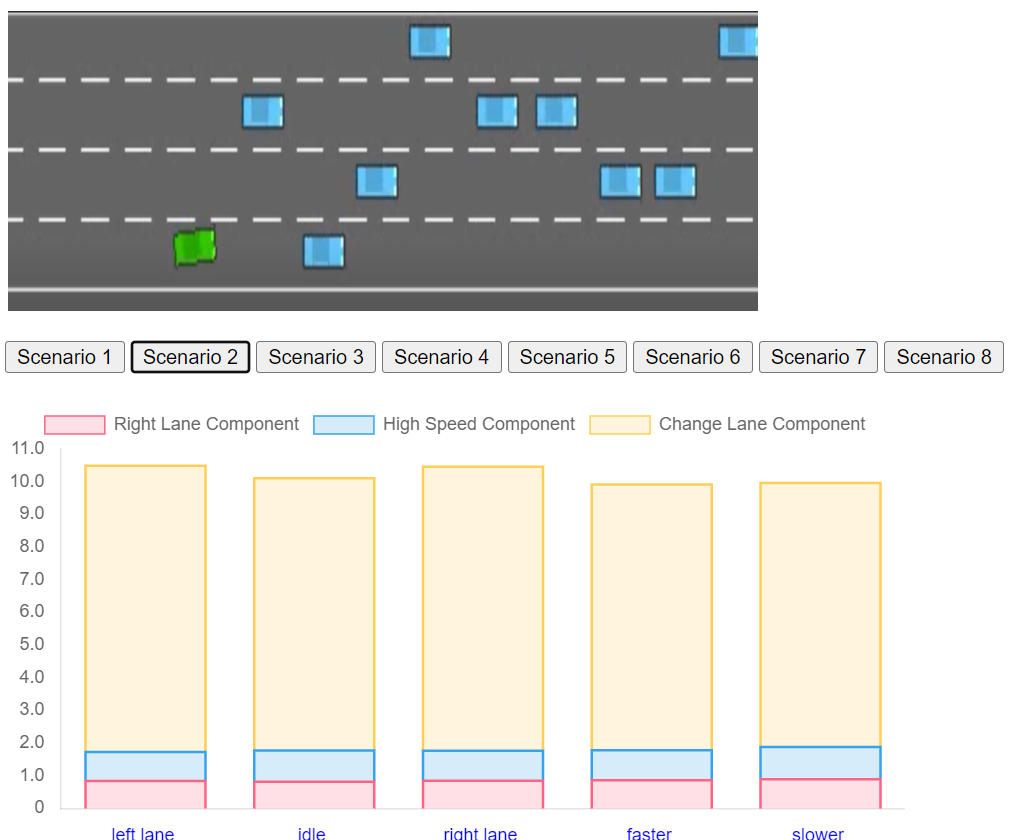
\includegraphics[width=0.49\linewidth]{example_from_survey.PNG}
\hfill
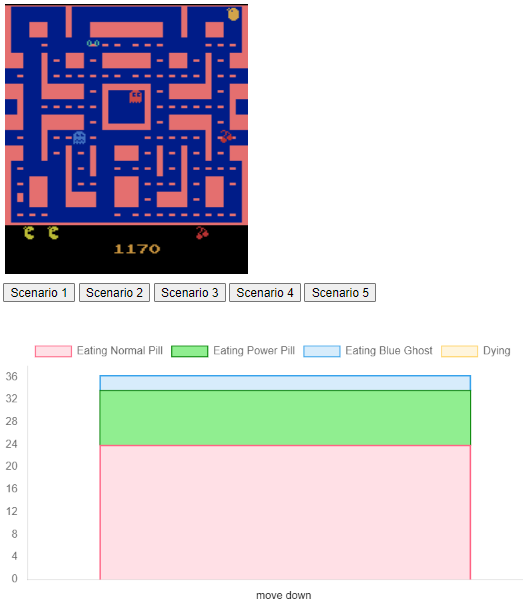
\includegraphics[width=0.39\linewidth]{Survey_example_Pacman.PNG}
\caption{Screenshots from our two experiments. The upper part of each screenshot shows a specific state (``Scenario 2'') extracted from an agent's behavior. The bottom part shows the reward bars corresponding to the state shown above. For each action (shown on the x-axis) the Q-values of the different reward components (depicted in different colors) are shown (y-axis). For Pacman, only the reward bar for the agent's chosen action is shown. Users could switch to different states by choosing a scenario from the list. The states (scenarios) were chosen based on the summary method (HIGHLIGHTS or frequency-based). For conditions without local explanation, the reward bars were omitted and each scenario showed a short video.}

\label{fig:example_from_survey}
\vspace{-0.2cm}
\end{figure}


\section{Empirical Methodology}
To evaluate the benefits of integrating HIGHLIGHTS with reward decomposition as well as their respective contributions to users' understanding of agents' behavior, we conducted two user studies in which participants were asked to evaluate the preferences of different agents. 
We hypothesized that the combined explanations would best support participants' ability to correctly identify agents' preferences and that both the local and global explanations would be better than the baseline information. 


\subsection{Experimental Environments and Agent Training}
\label{sec:exp_domains}
\subsubsection{Highway Environment}
We used a multi-lane Highway environment (shown in the top part of Figure \ref{fig:example_from_survey}) for our first experiments.
In the environment, the RL agent controls the green vehicle. The objective of the agent is to navigate a multi-lane highway while driving alongside other (blue) vehicles. Positive rewards can be given for each of the following situations: changing lanes (CL), speeding up (SU), and moving to the right-most lane (RML) (the environment assumes the convention of driving on the right). 
Therefore we use three reward components, corresponding to the aforementioned situations, for the reward decomposition. 
We trained the agents as described in Section \ref{sec:background}.
The network input is an array of size 25 (5X5) that represents the state. The input layer is followed by two fully connected hidden layers of length 256. The last of these two layers is connected to three heads. Each head consists of a linear layer and outputs a Q-value vector of length of 5 that contains the following: lane left, idle, lane right, faster, slower.
We trained four RL agents which differ in their policies:

(1) The Good Citizen -  The highest reward for being in the right lane, next to change lane, and lastly to speed up

(2) Fast And Furious - The highest reward for speeding up, then changing lanes, and lastly being in the right-most lane

(3) Dazed and Confused - The highest reward for changing lanes, next to be in the right-most lane, and lastly to speed up

(4) Basic - Reward for being in the right-most lane

Common to all agents, when crashing a negative reward of -3 is given, and no future rewards can be obtained due to ending the episode. 
The precise settings of the rewards for the different agents that we used are summarized in Table \ref{tab:reward setting}.
Each agent was trained for 2,000 episodes and each episode consists of 80 steps (or fewer if the agent crashed). 
Our implementation is based on two open source repositories: the Highway environment and an implementation of double DQN.\footnote{\url{https://github.com/eleurent/highway-env}, \url{https://github.com/eleurent/rl-agents}}


\begin{table}
\caption{Highway environment. Settings of the four agents.}
\label{tab:reward setting}
\parbox{.45\linewidth}{
    \centering
    \begin{tabular}{c|c c c c }
        \hline
         Agent & CL  & SU & RML  \\
           & reward & reward& reward \\
        \hline
        The Good Citizen & 3 & 1 & 8  \\
         Fast and Furious & 5 & 8 & 1  \\
        \hline
    \end{tabular}
    }
     \hfill
\parbox{.5\linewidth}{
    \centering
    \begin{tabular}{c|c c c c }
        \hline
          Agent & CL  & SU & RML  \\
           & reward & reward& reward \\
        \hline
Dazed and Confused & 8 & 1 & 5 \\        
         Basic & 0 & 0 & 15 \\
        \hline
    \end{tabular}
    }
\end{table}

The state importance definition for HIGHLIGHTS in the Highway environment is: $I(s) = \max\limits_{a} Q^{\pi}_{(s,a)}- \min\limits_{a}Q^{\pi}_{(s,a)}$, as used in the original HIGHLIGHTS implementation~\cite{amir2018highlights}. 
According to this formulation, a state is considered important if there is a large gap between the expected outcome of the best and worst action available to the agent in the state.
To extract the policy summaries, we ran 2,000 simulations of the trained agent and saved the traces.

\subsubsection{Pacman Environment}

In the second experiment, we used the Atari 2600 game MsPacman (Pacman for simplicity) contained in the Arcade Learning Environment \cite{bellemare2013ALE}.
For training the agents we build upon the Double DQN implementation in OpenAI baselines \cite{baselines}.
The network architecture is the same as used in \cite{mnih2015human}, which consists of 3 convolutional and 2 fully connected layers, and uses pre-processed pixel values as input.
We implemented reward decomposition (HRA) by sharing the convolutional layers but training individual fully connected layers for each reward component.
Our implementation can be found online.\footnote{\url{https://github.com/hcmlab/baselines/tree/reward\_decomposition}}

In the game, Pacman has to traverse a labyrinth while avoiding ghosts (see top of Figure~\ref{fig:example_from_survey}).
Based on the rules of the game, we used four different reward components ($|C|=4$) for the RL agent controlling Pacman: the agent receives a reward of 1 for eating normal pills (NP) and a reward of 5 for eating Power Pills (PP).
Additionally, after eating a PP, the ghosts turn blue and Pacman can eat them. 
The agent receives a reward of 20, 40, 80, or 160 for each blue ghost (BG) it eats successively.
Finally, the agent receives a reward of -10 for dying.
To get agents with distinct strategies, we used different weights for the reward components (see Table \ref{tab:reward setting pacman}).
Each agent was trained for 5 million steps.
In the Pacman environment, the values of the individual rewards do not directly correlate to the agents' preferences.
For example, the labyrinth contains a huge amount of normal pills compared to power pills and ghosts. 
Therefore, the agent with no specific reward component weights focuses very strongly on normal pills even though the reward value for individual normal pills is the lowest.
To determine what the agents preferred, we observed the Q-values and actions of each fully trained agent for several full games before running the experiment.
In total, we trained three different Pacman agents with the following preferences: 

(1) Normal Pill Agent - Highest preference for eating normal pills, next eating power pills and lastly eating blue ghosts

(2) Power Pill Agent - Highest preference for eating power pills, next eating normal pills and eating blue ghost has the same preference

(3) Blue Ghost Agent -  Highest preference for eating blue ghosts, next eating normal pills,  lastly eating power pills.

\begin{table}[t]
  \centering
  \caption{How each of the reward components was weighted for our Pacman agents.}
   \label{tab:reward setting pacman}
  \begin{tabular}{c|c c c c }
     \hline
         &  NP  &  PP & BG & Dying  \\
          & weights & weights & weights \\
       \hline
       Normal Pill Agent & 1 & 1 & 1 & 1  \\
         
        Power Pill Agent & 0.01 & 1 & 0.01 & 0.01 \\
        
       Blue Ghost Agent & 0.1 & 0.1 & 10 & 0.01  \\
       \hline
        
   \end{tabular}
   \vspace{-0.2cm}
\end{table}

We used HIGHLIGHTS-DIV to generate summaries for the Pacman agents. 
Compared to the basic HIGHLIGHTS algorithm, this approach additionally utilizes a similarity metric (Euclidean distance in our case) to avoid very similar states within the summaries \cite{amir2018highlights}.
Following Huber et al. ~\shortcite{huber2020local}, we calculated the importance as $I(s) = \max\limits_{a}Q^{\pi}_{(s,a)}- \operatornamewithlimits{second-highest}\limits_{a}Q^{\pi}_{(s,a)}$.
According to this formulation, a state is considered important if there is a large gap between the expected outcome of the best and second best action available to the agent in the state.
This was done since the Arcade Learning Environment implementation of Pacman contains several redundant actions. 
These redundant actions are often completely ignored by the agents and always have low Q-values.
To extract policy summaries, we ran the trained agent for 1,000 episodes after the training and recorded the traces.


\subsection{Study Design}
\emph{Experimental conditions}. We conducted two user studies to evaluate the impact of combining global and local explanations, as well as the effect of each method individually. Since local explanations are given for specific states, there must be some choice of which states to show the information for. Hence, as a baseline  approach, rather than using HIGHLIGHTS to select states, we used frequency sampling to generate summaries that choose states for the summary by uniform sampling from the traces of the agent, as used in the study by Huber et al. ~\cite{huber2020local}. Since each state has the same probability of being chosen, in practice states that appear more frequently are more likely to appear in the summary.
Therefore, this is equivalent to selecting states based on the likelihood of their appearance.
We assigned participants randomly to one of four different conditions:

\begin{itemize}
\item HIGHLIGHTS Summaries (H): In this condition, participants were shown summary videos that were generated by the HIGHLIGHTS algorithm.
We used a context window of 10 states that were shown before and after the chosen state and an interval size of 10 states to prevent directly successive states in the summary.

\item Frequency sampling summaries (FS): 
This condition contained videos similar to condition H, but the states in the middle of the trajectories were chosen based on frequency sampling. 
Moreover, to ensure that the summary is not particularly good or particularly bad we created 10 different summaries of this form for the Highways environment and 5 for Pacman.

\item HIGHLIGHTS + reward decomposition (H+RD): 
Since interpreting reward decomposition takes some time, we did not show videos in this condition.
Instead, participants were only shown the most ``important'' state of each trajectory.
This means that they did not get the context of that state as the video summaries provide.
However, the chosen states were the same states that appeared in the middle of the videos in condition H.
Each chosen state was shown using an image alongside a  bar plot that represents the Q-values of the different reward components. 
In the Highway environment, the bar plot was shown for each available action in the chosen state, as shown in Figure \ref{fig:example_from_survey}. 
Since Pacman contains ambiguous actions, we only showed the bar plot for the agents' chosen action in this environment.

\item Frequency sampling summaries + reward decomposition (FS+RD):
This condition was the same as condition H+RD but the shown states were the same states that were uniformly sampled for the middle of the trajectories in the FS condition.

\end{itemize}

Following ~\cite{huber2020local}, we set the size of the summaries for Pacman to $k=5$.
For the Highway environment, we used $k=8$.
Therefore, all participants were shown a summary of the agent's behavior that is composed of 5 or 8 different videos or images regarding the specific agent depending on the environment.


\emph{Procedure.} At first, participants were given an explanation regarding the environment (Highway or Pacman). 
Second, they were given a brief explanation about reinforcement learning and specifically about q-values in layperson vocabulary.
In particular, they were told that the agents are maximizing their future total score by taking into account both immediate points as well as points for future actions. 
Lastly, depending on the condition, participants were given information about the type of explanation they will see and an example explanation.
At the end of each instructions phase, the participants were asked to complete a quiz and were only allowed to proceed after answering all questions correctly.
Participants were compensated as follows: they received a \$3 base payment and an additional bonus of 10 cents for each correct answer in the Highway environment and a 30 cent bonus for identifying the preferences of each of the agents correctly in the Pacman environment.

\emph{Task.} 
The participant's task was to assess the preferences of the different agents.
To avoid learning effects, the ordering of the agents was randomized. 
Specifically, participants were asked to rank which of each pair of reward components (e.g., high speed vs. driving in the right lane in the Highway environment or  eating power pills vs. eating normal pills in the Pacman environment) the agent prioritizes or whether it is indifferent between the two options.
If participants have a correct mental model of the agents' strategy, they should be able to rank the different reward components according to the agents' priorities.

Participants were then asked to rate their confidence in each of their answers on a Likert scale from 1 (``not confident at all'') to 5 (``very confident'') and to describe their reasoning in a free-text response.
Lastly, participants rated their agreement on a 7-point Likert scale with the following items adapted from the explanation satisfaction questionnaire proposed by Hoffman et al.~\cite{hoffman2018metrics}
:\begin{enumerate}
\item The videos$\backslash$graphs helped me recognize agent strategies
\item The videos$\backslash$graphs contain sufficient detail for recognizing agent strategies
\item The videos$\backslash$graphs contain irrelevant details 
\item The videos$\backslash$graphs were useful for the tasks I had to do in this survey
\item The specific scenarios shown in the videos$\backslash$images were useful for the tasks I had to do in this survey.
\end{enumerate}
\emph{Participants}. We recruited participants through Amazon Mechanical Turk (N = 164 for each environment). We excluded participants who did not answer the attention question correctly, as well as participants who completed the survey in less than two standard deviations from the mean completion time in their condition.
After screening, we had 127 and 159 participants in the Highway environment and the Pacman environment respectively (mean age = 36 years for both environments, 58 and 88 female in the Highway environment and the Pacman environment respectively,  all from the US, UK, or Canada).

\section{Results}
To measure participants' ability to asses the agents' preferences, we calculated the mean fraction of correct reward component comparisons, i.e., their correctness rate, for each condition (see Figure~\ref{fig:results}).
We tested our hypotheses using the non-parametric, one-sided Mann-Whitney $U$ test. Only when comparing the individual explanation conditions H and FS+RD, we used a two-sided test since we did not have a hypothesis as to which method will be better.

\begin{figure}[t]
\begin{minipage}{0.49\linewidth}
\centering
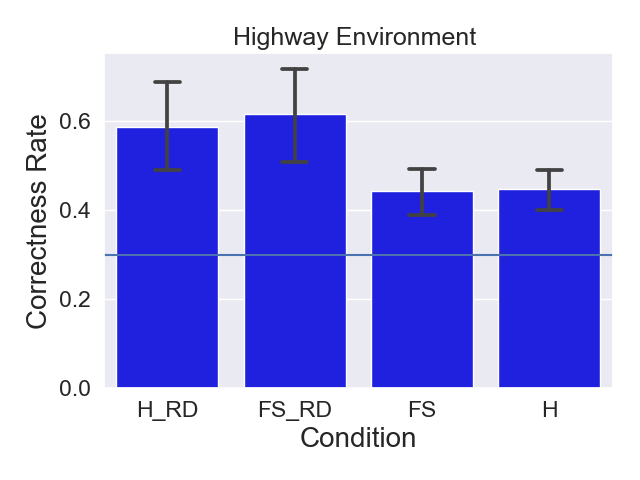
\includegraphics[width=0.49\linewidth]{myplot_highway.png}
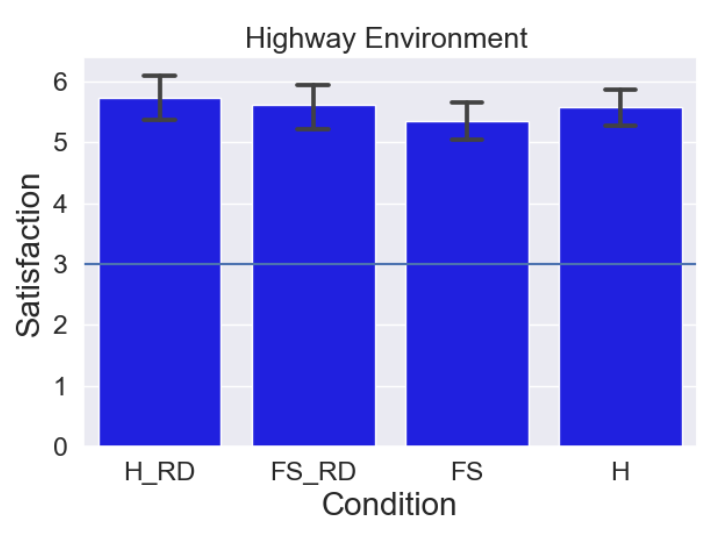
\includegraphics[width=0.49\linewidth]{Highway_env_satisfaction.png}

(A)
\end{minipage}
\begin{minipage}{0.49\linewidth}
\centering
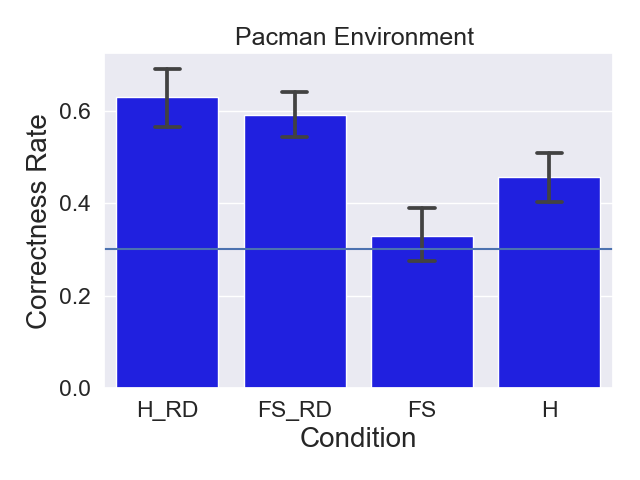
\includegraphics[width=0.49\linewidth]{myplot_all.png}
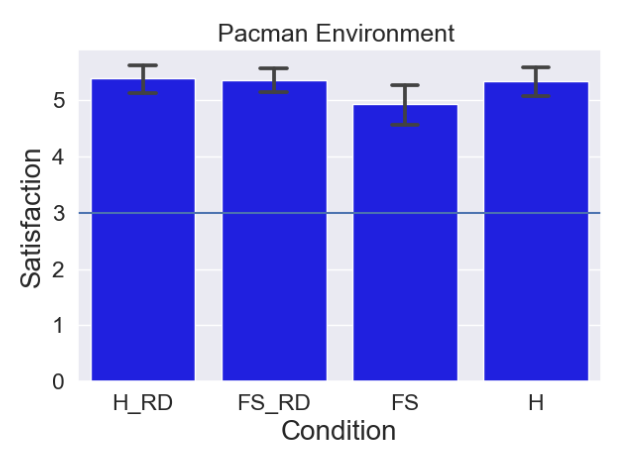
\includegraphics[width=0.49\linewidth]{Pacman_env_satisfaction.png}

(B)
\end{minipage}
\vspace{-0.3cm}

\caption{Participants' mean correctness rate in identifying the preferences averaged over all agents and participants' explanation satisfaction by conditions in the Highway (A) and in the Pacman (B) environment. The error bars show the 95\% CI. }
\label{fig:results}
\vspace{-0.6cm}
    %\vspace{3pt}
\end{figure}

\textbf{We found that reward decomposition improved participants' ability to asses the agents' preferences in both environments}.
In the Highway environment, the combination of FS+RD 
led to significantly improved performance compared to FS 
(FS+RD vs. FS: $U$=$736$, $p$=$0.014$; FS+RD vs. H: $U$=$791$, $p$=$0.017$). 
Similarly, H+RD 
led to significantly improved performance compared to FS and H ($U$=$532$, $p$=$0.014$ and $U$=$571$, $p$=$0.018$, respectively).
Similarly, in the Pacman environment, the combination of FS+RD 
significantly improved participants' performance compared to FS or H
($U$=$1187$ and $U$=$1176$ respectively, $p$$<$$0.001$ for both) and participants in the H+RD condition 
performed better compared to FS and H ($U$=$1286$ and $U$=$1332$ respectively, $p$$<$$0.001$ for both).
Some of the participants explicitly referred to reward decomposition as being helpful for the task, e.g., ``In each of the scenarios the graph clearly shows the preference for normal pills followed by eating power pills. Eating ghosts was a minor section on the graph.''

\textbf{The HIGHLIGHTS summaries only contributed to participants' mental model of the agents in the Pacman environment}. 
Here, there was a significant difference between condition H and condition FS ($U$=$935$, $p$=$0.002$). In some explanations given by participants, it seemed that the HIGHLIGHTS summary displayed information that was useful for inferring preference, e.g., one participant wrote ``the pacman would go for a power pill, eat it and turn around'' when explaining their answers about the Power Pill agent preferences.

\textbf{In both environments, the combined explanation did not outperform reward decomposition alone}.
There were no significant differences between H+RD and FS+RD in either of the environments when aggregated across all agents.
However, in the Highway environment, our results indicate that the combination of H+RD helped asses the agent's preferences when the difference between the reward types was minor. 
For example, when assessing the agent ``Fast and Furious'' that was trained according to the rewards of 8 points for speed up vs. 5 points for changing lanes, participants who were shown H+RD succeeded about half of the times ($M$=$0.55$, $95\%$ $CI$=$(0.41,0.69)$) compared to participants in conditions FS+RD, FS or H that had a lower success rate ($M$=$0.44$, $95\%$ $CI$=$(0.34,0.54)$; $M$=$0.18$, $95\%$ $CI$=$(0.03,0.33)$; $M$=$0.26$, $95\%$ $CI$=$(0.1,0.42)$, respectively). 
Similarly, for the BG agent in Pacman, there was only a small difference between the Q-values for the blue ghosts and normal pills. 
Participants in conditions H ($M$=$0.3$, $95\%$ $CI$=$(0.2,0.5)$) and H+RD ($M$=$0.31$, $95\%$ $CI$=$(0.17,0.46)$) were better at correctly identifying the blue ghost as more important than the participants in conditions FS+RD ($M$=$0.2$, $95\%$ $CI$=$(0.17,0.46)$)  and FS ($M$=$0.12$, $95\%$ $CI$=$(0,0.23)$).
This indicates that even though our overall results do not show that the combination of H+RD is significantly better, there were cases in which this combination helped.

\textbf{In general, while participants' objective performance was better with RD compared to video-based policy summaries, this did not lead to an increase in subjective measures}.
In the Highway environment, participants' confidence and satisfaction ratings were above the neutral rating ($>3$) but there was no difference between the conditions.
In the Pacman environment, the confidence and satisfaction values of participants were also above neutral (see Figure \ref{fig:results}).
However, here the explanation conditions FS+RD, H+RD, and H had higher mean satisfaction ratings ($M$ between $5.34$ and $5.39$) than the baseline condition (condition FS with $M$=$4.93$).


\section{Discussion}

In previous work, HIGHLIGHTS summaries were integrated with saliency maps, but a user study showed that saliency maps did not provide much benefit to users' understanding of agent behavior~\cite{huber2020local}. We hypothesized that reward decomposition may be more beneficial for several reasons. First, saliency maps describe what features of the state the agent pays attention to, but it is often hard to infer how this information affects the agent's decisions, especially for laypeople. Reward decomposition has the benefit of explicitly describing what values the agent expects to get in a way that reflects its preferences for different reward components. Moreover, saliency maps are a post-hoc method and may not be faithful to the underlying model~\cite{rudin19,huber2022benchmarking} while reward decomposition values are learned through the agent's training and reflect its true decision-making policy. 
Another difference between our integration of global and local information and the one used in the study by Huber et al.~\shortcite{huber2020local} is the use of static images rather than videos. We chose this approach based on the findings from their study which identified the use of videos as one possible limitation, as the local information is harder to discern when looking at dynamic videos.


Our studies showed a fairly limited contribution of HIGHLIGHTS summaries to participants' performance compared to prior works~\cite{amir2018highlights,huber2020local}, with improved performance observed only in some scenarios in the Pacman environment. A possible explanation for the limited contribution of HIGHLIGHTS is that the experimental task may have been particularly suited to reward decomposition. Since reward decomposition was already highly effective in conveying agent preferences, the selection of states for the summary was less important. We further hypothesize that HIGHLIGHTS summaries were not better than frequency-based summaries in the Highway environment since the environment is somewhat limited in terms of agent behaviors.

\section{Conclusion and Future Work}
This paper presented a new approach for describing the behavior of RL agents, which integrates HIGHLIGHTS, a global policy summary, with local reward decomposition. We conducted user studies in two environments to evaluate the contribution of this approach to people's ability to analyze agent preferences. Our results show that reward decomposition was particularly helpful for this task and that HIGHLIGHTS also led to improvement in participants' performance, but only in certain situations. 

The fact that the intrinsic reward decomposition method in our work outperforms the post-hoc saliency maps used in a similar experiment \cite{huber2020local} empirically reaffirms the recommendation by Rudin \cite{rudin19} to use intrinsic explanation methods whenever possible.
Furthermore, based on the difference between our study and the one by Huber et al. \cite{huber2020local}, who showed their local saliency maps on videos instead of static states, future combinations of local explanations and global policy summarization should provide the local explanation on static states.
This allows users to discern the information within the explanation. 

The finding that HIGHLIGHTS only improved participants' performance in the Pacman environment indicates that the usefulness of policy summaries may depend on the complexity of behaviors that agents may deploy in a domain.
Future work should explore how the characteristics of different environments affect the usefulness of alternative explanation methods.

Another notable finding is that the use of different explanation methods did not result in substantial differences in subjective measures like explanation satisfaction. This finding emphasizes the importance of using objective performance measures for XAI, while also showing the need for future work on how we can increase the usability of explanatory systems.


\subsubsection{Acknowledgements} 
 We thank Julian Stockmann and Simone Pompe for their help with implementing HRA for MsPacman.

%
% ---- Bibliography ----
%
% BibTeX users should specify bibliography style 'splncs04'.
% References will then be sorted and formatted in the correct style.
%
% \small
\bibliographystyle{splncs04}
\bibliography{refs}
%


\end{document}
